\chapter{Laboratorio 1: \\Power Estimation: probabilistic techniques}
\section{Probability and Activity Calculation: Simple Logic Gates}
Durante la prima parte dell'esercitazione è stato richiesto di calcolare la probabilità di avere '1' logico in uscita di alcuni gate elementari, con la relativa Switching Activity.
\begin{figure}[!htb]
	\centering
	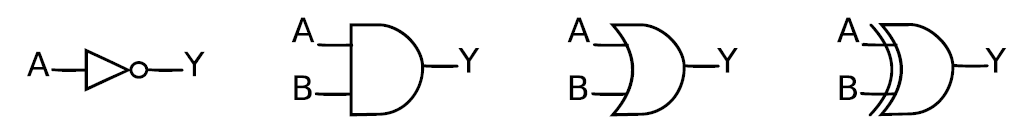
\includegraphics[scale=0.8]{immagini/gate}
	\caption{\textit{Gate elementari}}
	\label{fig1_1}
\end{figure} \\
La probabilità di '1' logico è stata stimata semplicemente andando a valutare il rapporto fra il numero di possibili combinazioni con '1' logico diviso il numero di combinazioni totali. Invece per il calcolo della Switching Activity è stata utilizzata la formula vista a lezione:
\begin{center}
	$ A=E_{SW}=P_{1}P_{0}+P_{1}P_{0}=2P_{1}(1-P_{1}) $
\end{center}
Dove $P_{1}$ e $P_{0}$ sono le probabilità di avere '1' e '0' logici in uscita dalla mia porta. \\
Di seguito si riportano i procedimenti matematici per ottenere le probabilità e le Switching Activity dei gate elementari visti in Figura \ref{fig1_1}.\\
\begin{itemize}
	\item \textit{Inverter} \\
	$P_{1}(Y)=P_{0}(A)=\frac{1}{2}$ \\
	$P_{0}(Y)=P_{1}(A)=\frac{1}{2}$ \\
	$E_{SW}=2P_{1}(Y)(1-P_{1}(Y))=2\frac{1}{2}\frac{1}{2}=\frac{1}{2}$\\
	\item \textit{AND} \\
	$P_{1}(Y)=P_{1}(A)P_{1}(B)=\frac{1}{2}\frac{1}{2}=\frac{1}{4}$ \\
	$E_{SW}=2P_{1}(Y)(1-P_{1}(Y))=2\frac{1}{4}\frac{3}{4}=\frac{3}{8}$\\
	\item \textit{OR} \\
	$P_{1}(Y)=P_{1}(A)P_{1}(B)+P_{0}(A)P_{1}(B)+P_{1}(A)P_{0}(B)=\frac{1}{2}\frac{1}{2}+\frac{1}{2}\frac{1}{2}+\frac{1}{2}\frac{1}{2}=\frac{3}{4}$ \\
	$E_{SW}=2P_{1}(Y)(1-P_{1}(Y))=2\frac{3}{4}\frac{1}{4}=\frac{3}{8}$\\
	\item \textit{XOR} \\
	$P_{1}(Y)=P_{1}(A)P_{0}(B)+P_{0}(A)P_{1}(B)=\frac{1}{2}\frac{1}{2}+\frac{1}{2}\frac{1}{2}=\frac{1}{2}$ \\
	$E_{SW}=2P_{1}(Y)(1-P_{1}(Y))=2\frac{1}{2}\frac{1}{2}=\frac{1}{2}$\\
\end{itemize}
Per maggiore chiarezza, i risultati sono raccolti nella Tabella \ref{Tab1_1}. \\
\begin{table}[!h]\footnotesize
	\centering
	\begin{tabular}{|c|c|c|c|c|}
		\hline
		 & \textbf{INVERTER}& \textbf{AND}& \textbf{OR} &\textbf{XOR}\\
		\hline
		$P_{1}(Y)$ & $1/2$  & $1/4$& $3/4$&$1/2$\\
		\hline
		$E_{SW}$& $1/2$ &$3/8$&$3/8$& $1/2$\\
		\hline
	\end{tabular}
	\caption{\textit{Risultati ottenuti manualmente}}
	\label{Tab1_1}
\end{table}\\
In seguito, tramite il programma \textit{ModelSim} è stato analizzato il numero di toogle delle varie porte utilizzando un testbench sviluppato appositamente dai docenti. Si è andato a variare il numero di colpi di clock, come richiesto dalla traccia ed in seguito si sono comparati i valori ottenuti dalla simulazione con ciò che si era calcolato manualmente.\\
Tramite appositi comandi di Modelsim (\textbf{-power report}), sono stati stilati dei report relativi ad una stima delle commutazioni delle varie porte, della quale se ne riporta un esempio in Figura \ref{fig1_2}. Questi report consentono di stimare l'attività delle porte come verrà descritto in seguito.\\
\begin{figure}[!htb]
	\centering
	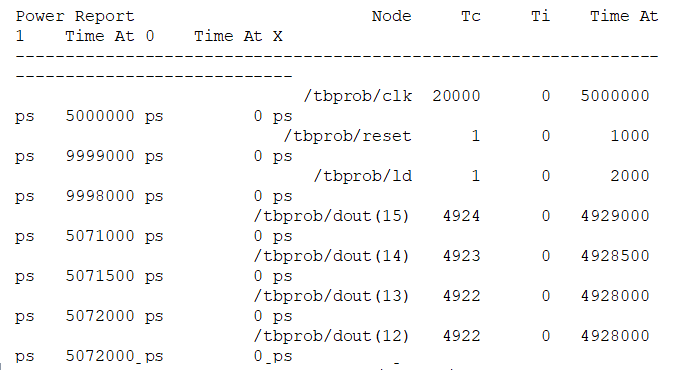
\includegraphics[scale=1]{immagini/fig1_2}
	\caption{\textit{Probabilità e Switching Activity stimati dal simulatore}}
	\label{fig1_2}
\end{figure} \\
Si riportano nella tabella \ref{tab1}, i risultati ottenuti dalle varie simulazioni.
\begin{table}[!h]\footnotesize
	\centering
	\begin{tabular}{|c|c|c|c|c|}
		\hline
		\textbf{Tc(CK)} & \textbf{Tc(INV)}& \textbf{Tc(AND)}& \textbf{Tc(OR)} &\textbf{Tc(XOR)}\\
		\hline
		20 & 1  & 5& 4&4\\
		\hline
		200 &  43 &40&42& 44\\
		\hline
		2000& 533& 418&352&470\\
		\hline
		20000& 4916& 3606&3784&4876\\
		\hline
	\end{tabular}
	\caption{\textit{Risultati simulazione}}
	\label{tab1}
\end{table}\\
Dai seguenti valori è facile ricavare i valori di Switching Activity simulate, in quanto si possono stimare da:
\begin{center}
	$ A=E_{SW}=\frac{Tc(PORT)}{T_{CLK}} $
\end{center}
Come ci si aspettava, essendo la Switching Activity il numero di toggle avvenuti in un periodo, i valori delle simulazioni vengono molto simili ai valori calcolati analiticamente. Aumentando il tempo di simulazione, i valori di Switching Activity diventano sempre più precisi, arrivando ad avere un errore tra 0.01-0.5. I vari valori sono stati calcolati e raccolti nella Tabella \ref{Tab1_2}
\begin{table}[!h]\footnotesize
	\centering
	\begin{tabular}{|c|c|c|c|c|}
		\hline
		\textbf{$N_{CLOCK}$} & \textbf{$E_{SW}(INV)$}& \textbf{$E_{SW}(AND)$}& \textbf{$E_{SW}(OR)$} &\textbf{$E_{SW}(XOR)$}\\
		\hline
		10 & 0.1  & 0.5& 0.4&0.4\\
		\hline
		100 &  0.43 &0.40&0.42& 0.44\\
		\hline
		1000& 0.533& 0.418&0.352&0.470\\
		\hline
		10000& 0.492& 0.36&0.378&0.487\\
		\hline
	\end{tabular}
	\caption{\textit{Switching activities calcolate}}
	\label{Tab1_2}
\end{table}\\

\section{Probability and Activity Calculation: Half and Full adder}
Nella seconda parte dell'esercitazione viene richiesto di analizzare le probabilità e la Switching Activity di un Half Adder e di un Full Adder, sia per quanto riguarda l'uscita $S$ sia per quanto riguarda il carry out $C_{OUT}$, dei quali se ne riporta lo schema circuitale rispettivamente in Figura \ref{half_adder} e \ref{full_adder}.
\begin{figure}[!htb]
	\centering
	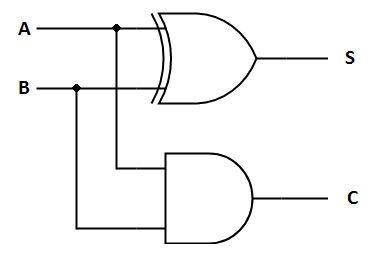
\includegraphics[scale=0.4]{immagini/half_adder}
	\caption{\textit{Schema circuitale Half Adder}}
	\label{half_adder}
\end{figure} \\
\begin{figure}[!htb]
	\centering
	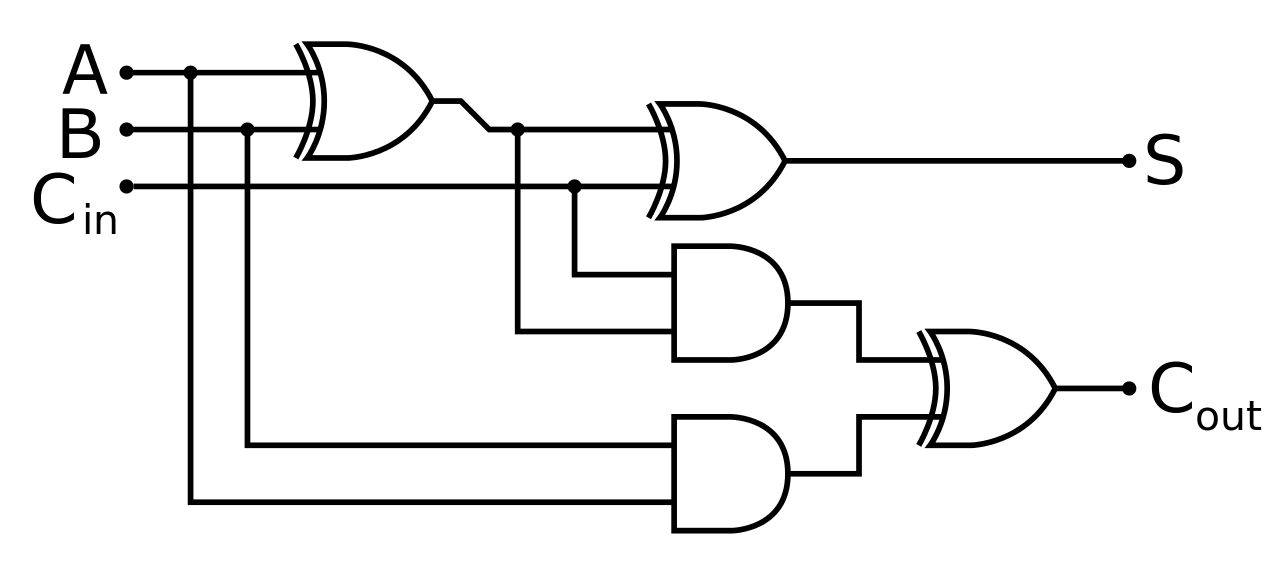
\includegraphics[scale=0.2]{immagini/full_adder}
	\caption{\textit{Schema circuitale Full Adder}}
	\label{full_adder}
\end{figure} \\
Il calcolo è stato effettuato in entrambi in casi, analizzando il blocco come un unico gate e andando a studiare la rispettiva Tavola di Verità. Anche in questa sezione, si considerano gli ingressi equiprobabili e scorrelati, con probabilità $P('input')=0.5$ Il risultato è stato il seguente:\\
\begin{itemize}
	\item \textit{Half-Adder} \\
	$P_{1}(S)=P_{1}(A)P_{0}(B)+P_{0}(A)P_{1}(B)=\frac{1}{2}\frac{1}{2}+\frac{1}{2}\frac{1}{2}=\frac{1}{2}$ \\
	$E_{SW}(S)=2P_{1}(S)(1-P_{1}(S))=2\frac{1}{2}\frac{1}{2}=\frac{1}{2}$\\
	$P_{1}(C_{OUT})=P_{1}(A)P_{1}(B)=\frac{1}{2}\frac{1}{2}=\frac{1}{4}$ \\
	$E_{SW}(C_{OUT})=2P_{1}(C_{OUT})(1-P_{1}(C_{OUT}))=2\frac{1}{4}\frac{3}{4}=\frac{3}{8}$\\
	\item \textit{Full-Adder} \\
	$P_{1}(S)=
	P_{0}(A)P_{0}(B)P_{1}(C_{IN})+
	P_{0}(A)P_{1}(B)P_{0}(C_{IN})+
	P_{1}(A)P_{0}(B)P_{0}(C_{IN})++
	P_{1}(A)P_{1}(B)P_{1}(C_{IN})
	=\frac{1}{2}\frac{1}{2}\frac{1}{2}+
	\frac{1}{2}\frac{1}{2}\frac{1}{2}+
	\frac{1}{2}\frac{1}{2}\frac{1}{2}+
	\frac{1}{2}\frac{1}{2}\frac{1}{2}=\frac{1}{2}$ \\
	$E_{SW}(S)=2P_{1}(S)(1-P_{1}(S))=2\frac{1}{2}\frac{1}{2}=\frac{1}{2}$\\
	$P_{1}(C_{OUT})=
	P_{0}(A)P_{1}(B)P_{1}(C_{IN})+
	P_{1}(A)P_{0}(B)P_{1}(C_{IN})+
	P_{1}(A)P_{1}(B)P_{0}(C_{IN})++
	P_{1}(A)P_{1}(B)P_{1}(C_{IN})+
	=\frac{1}{2}\frac{1}{2}\frac{1}{2}+
	\frac{1}{2}\frac{1}{2}\frac{1}{2}+
	\frac{1}{2}\frac{1}{2}\frac{1}{2}+
	\frac{1}{2}\frac{1}{2}\frac{1}{2}=\frac{1}{2}$ \\
	$E_{SW}(C_{OUT})=2P_{1}(C_{OUT})(1-P_{1}(C_{OUT}))=2\frac{1}{2}\frac{1}{2}=\frac{1}{2}$\\
\end{itemize}
I risultati sono sintetizzati nella Tabella \ref{Tab1_4}
\begin{table}[!h]\footnotesize
	\centering
	\begin{tabular}{|c|c|c|c|c|}
		\hline
		& $P(S=1)$&$P(C_{OUT}=1)$& $E_{SW}(S=1)$&$E_{SW}(C_{OUT}=1)$\\
		\hline
		\textbf{Half-Adder} & 1/2  & 1/4&1/2&3/8\\
		\hline
		\textbf{Full-Adder} &  1/2 &1/2&1/2& 1/2\\
		\hline
	\end{tabular}
	\caption{\textit{Risultati ottenuti manualmente}}
	\label{Tab1_4}
\end{table}\\

\noindent In seguito si sono calcolate, sempre analiticamente, le probabilità di uscita con le rispettive switching activities del Ripple Carry Adder, riportato in Figura \ref{ripple}, utilizzando i dati calcolati in precedenza per il singolo Full-Adder. Anche per questo calcolo iniziale gli ingressi sono stati considerati scorrelati ed equiprobabili.
\begin{figure}[!htb]
	\centering
	\includegraphics[scale=0.9]{immagini/ripple}
	\caption{\textit{Ripple Carry Adder}}
	\label{ripple}
\end{figure} \\
I risultati sono riportati nella Tabella \ref{Tab1_3}.\\
\begin{table}[!h]\footnotesize
	\centering
	\begin{tabular}{|c|c|c|c|c|c|c|c|c|}
		\hline
		&\textbf{FA7}& \textbf{FA6}& \textbf{FA5} &\textbf{FA4}&\textbf{FA3}&\textbf{FA2}&\textbf{FA1}&\textbf{FA0}\\
		\hline
		$P(S=1)$&1/2 &1/2&1/2&1/2&1/2&1/2&1/2&1/2\\
		\hline
		$E_{SW}$&1/2&1/2&1/2&1/2&1/2&1/2&1/2&1/2\\
		\hline
	\end{tabular}
	\caption{\textit{Probabilità e Switching Activity stimati manualmente con ingressi equiprobabili}}
	\label{Tab1_3}
\end{table}
\\
\noindent Se invece si considerano gli ingressi non equiprobabili, ma comunque scorrelati, con probabilità rispettivamente $P(A='1')=0.4$ e $P(B='1')=0.6 $, ci si aspetta un risultato differente, infatti le probabilità dei nodi di uscita trovate sono: $P(S ='1')=0.52$ e $P(Co ='1')=0.24$ \\
In seguito, tramite il programma \textit{ModelSim} è stato simulato il Ripple Carry Adder utilizzando un testbench sviluppato appositamente dai docenti e utilizzando le procedure viste nel paragrafo 1.1.\\
La simulazione viene fatta andando ad inserire dei ritardi sulle uscite $S$ e $C_{OUT}$ dei singoli Full-Adder. Inizialmente si setta esclusivamente un ritardo di 25 ps esclusivamente sul segnale $S$, mentre in secondo luogo si introduce un ritardo uguale anche sul segnale di $C_{OUT}$.\\
Il testbench è stato costruito appositamente per assegnare ritardi diversi al bit di somma, DRCAS, e al bit di carry, DRCAC. Inoltre per garantire una simulazione generale si è utilizzato l'LFSR per generare ingressi randomici. Per una corretta visualizzazione dei risultati si è impostata una risoluzione di 1ps. Dopo aver visualizzato il power report, come fatto già in precedenza, si sono comparati i valori ottenuti dalla simulazione con ciò che si era calcolato manualmente, seguendo lo stesso ragionamento del punto precedente.\\
	\begin{figure}[!htb]
		\centering
		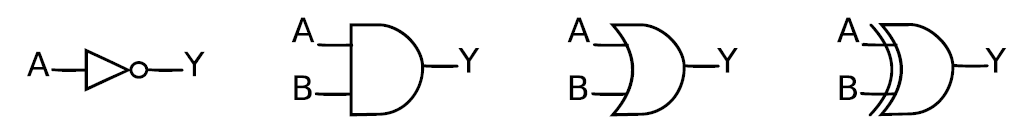
\includegraphics[scale=1]{immagini/gate}
		\caption{\textit{Power report}}
		\label{fig1_3}
	\end{figure} \\
	(cosa noto?) e bisogna mettere le waveforms?\\                                <- ATTENZIONE
Si è poi simulato il caso in cui i due ritardi riguardanti il bit di somma e il bit di carry fossero uguali, e anche per questo è stato visualizzato il power report.   
\begin{figure}[!htb]
		\centering
		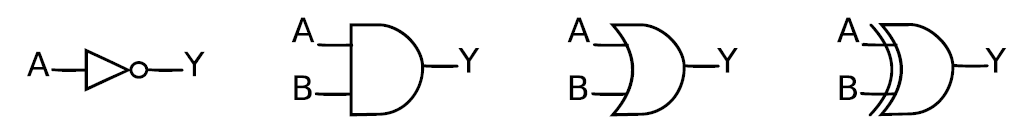
\includegraphics[scale=1]{immagini/gate}
		\caption{\textit{Power report con ritardi uguali}}
		\label{fig1_4}
	\end{figure} \\
	Da un analisi e confronto tra i risultati ottenuti manualmente e quelli ottenuti con le simulazioni, si nota come questi coincidano dato che avendo uguali ritardi, non riesco a simulare la presenza di eventuali glitch.\\
	In seguito si è calcolata la switching activity totale dei due sommatori, utilizzanso la seguente formula:
	\begin{center}
		$ A=\sum_{i=1}^{N-1}{A(S_i)} $  %<- risultato??
	\end{center}
What is the overhead computation of the second adder?  $<$- cioè? \\
Come ultima cosa è stato simulato il secondo testbench che ci è stato fornito, dove si simulava sempre un Ripple carry adder, ma questa volta in maniera puramente combinatoria.Analizzando i risultati, si può concludere come non avendo un segnale di temporizzazione, lavoro alla massima velocità ma ho la presenza di glitch.

\section{RCA synthesis and power analysis}
Nella seguente sezione dell'esercitazione è stata analizzata la potenza del sommatore RCA già analizzato in precedenza, tramite il software \textit{Synopsys}. Dopo aver analizzato ed elaborato i file che descrivono la struttura dell'RCA, il tutto è stato sintetizzato e sono stati raccolti i vari report relativi alla potenza.
Un primo report di potenza, riportato in Figura \ref{report_power1}, descrive i contributi di potenza relativi alle 8 istanze dei Full-Adder che compongono il somamtore RCA. \\
\begin{figure}[!htb]
	\centering
	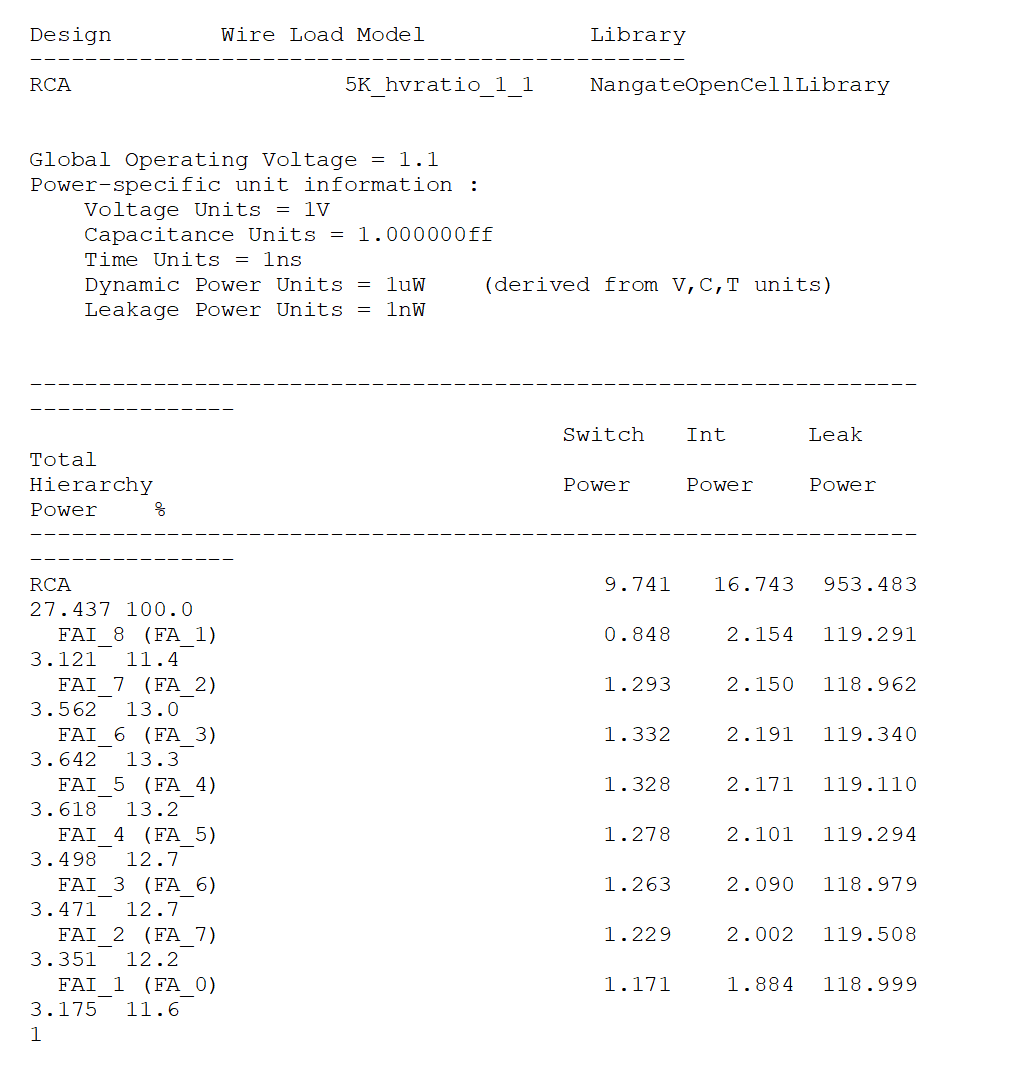
\includegraphics[scale=0.7]{immagini/report_power1}
	\caption{\textit{Power report}}
	\label{report_power1}
\end{figure}
\\
Come ci si aspettava, i contributi dei vari Full Adder sono tutti simili tra di loro, ad eccezione dell'istanza \textit{FAI\_8}: il motivo consiste nel fatto che il Carry Out dell'ultimo Full Adder non è connesso a nessun altra porta, dunque il carico da pilotare è decisamente minore.\\
Diventa ora interessante andare ad analizzare la singola istanza, per andare a valutare l'origine dei singoli contributi di potenza. Tramite il comando \textit{current\_instance FAI\_1} si va ad analizzare l'istanza relativa al primo Full Adder. Viene riportato il report in Figura \ref{reportFA1}.\\
\begin{figure}[!htb]
	\centering
	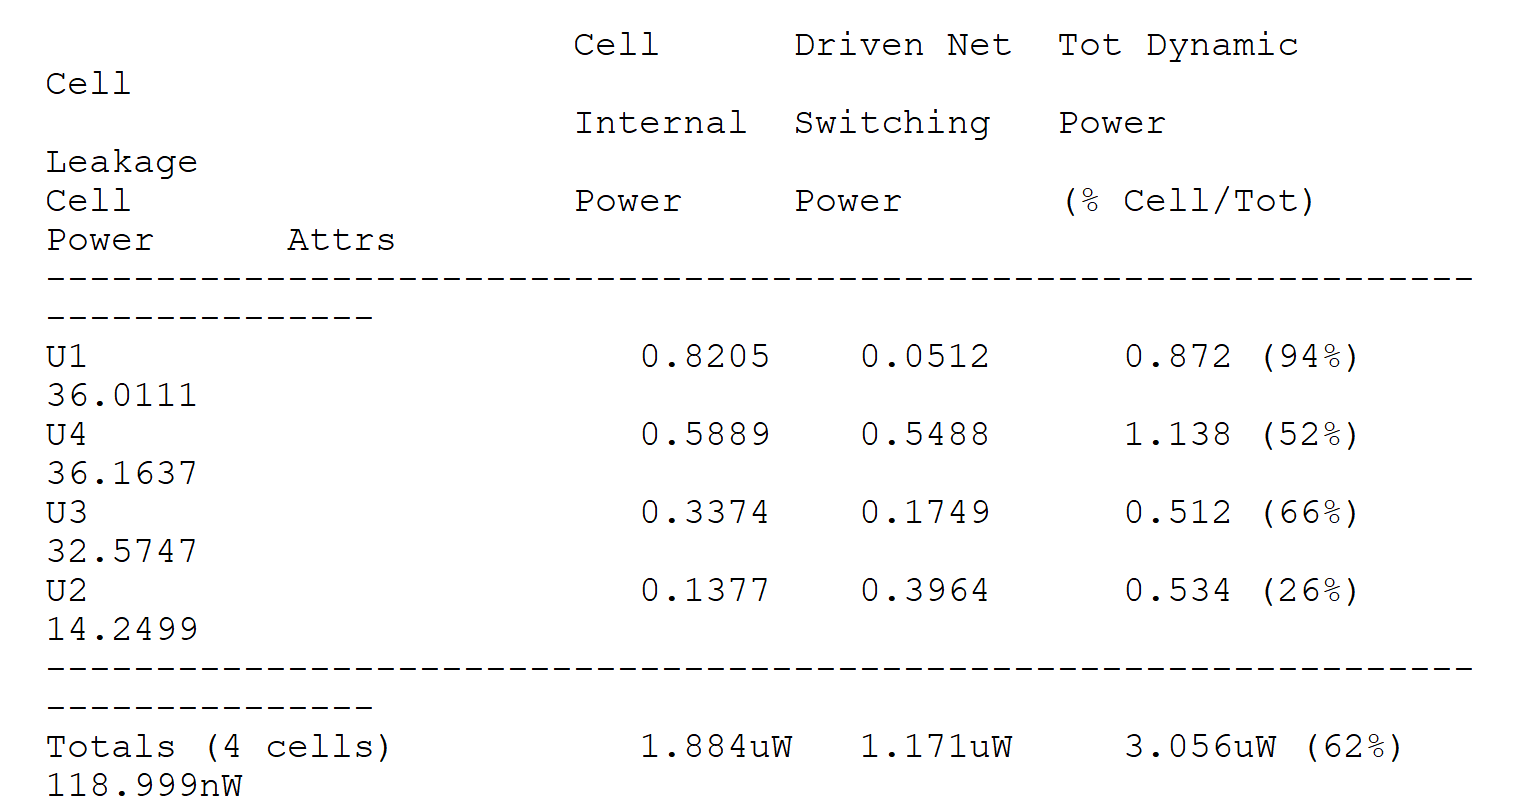
\includegraphics[scale=0.6]{immagini/reportFA1}
	\caption{\textit{Power report}}
	\label{reportFA1}
\end{figure}
\\
\\
\\
Come ci si aspettava i valori di potenza risultano assolutamente identici al report trovato in precendenza e riportato in Figura \ref{report_power1}.
Il passo successivo è comprendere come avvenga la stima della potenza dinamica (\textit{switching power}) dei singoli nodi del FA, dato che la potenza interna e quella di leakage dipendono solo dal gate e non dal circuito. Si utilizza a questo scopo il comando \textit{report\_power -net -verbose} e si riporta il report risultante in Figura \ref{verbose1}.
\begin{figure}[!htb]
	\centering
	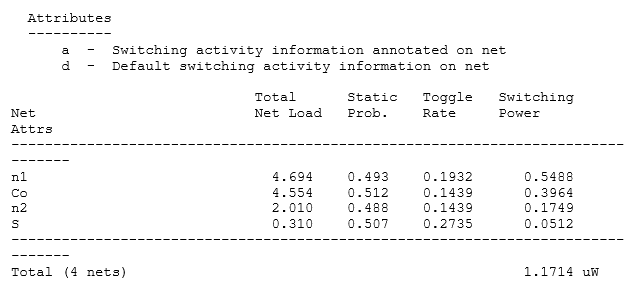
\includegraphics[scale=0.6]{immagini/verbose1}
	\caption{\textit{Power report current\_istance}}
	\label{verbose1}
\end{figure}
\\
Si può notare come la potenza dinamica consumata dal nodo di uscita S sia praticamente nulla, in quanto essa non deve pilotare alcun carico, a meno della potenza che il software considera per le varie capacità parassite. \\
Con questa analisi, il software si preoccupa anche di fare un'analisi probabilistica delle varie attività dei nodi. Dal report si può notare come siano assolutamenti concordi con i valori teorici trovati in precedenza.\\
Si ritorna ora al circuito complessivo, salendo di livello logico e si analizzano i nodi anche in questa situazione utilizzando lo stesso comando utilizzato in precedenza. Il report viene raffigurato in Figura \ref{verbose2}.
\begin{figure}[!htb]
	\centering
	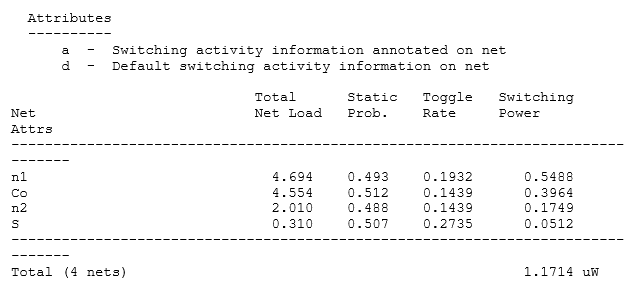
\includegraphics[scale=0.6]{immagini/verbose1}
	\caption{\textit{Power report}}
	\label{verbose2}
\end{figure}

\section{A simple MUX: glitch generation and propagation}
\begin{figure}[!htb]
	\centering
	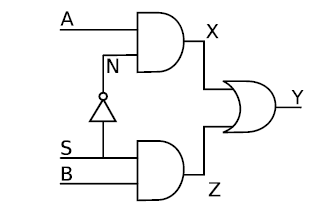
\includegraphics[scale=0.8]{immagini/mux}
	\caption{\textit{Power report}}
	\label{mux}
\end{figure}
\noindent Durante questa sezione, viene chiesto di analizzare il comportamento di un Multiplexer, riportato in Figura \ref{mux}, dove si assume che i ritardi delle varie porte elementari siano nulli, ad eccezione dell'Inverter che presenta un ritardo pari a 0,1 ns. Inizialmente si simula il circuito utilizzando \textit{ModelSim} e si riportano le one in Figura \ref{model_mux}.
\begin{figure}[!htb]
	\centering
	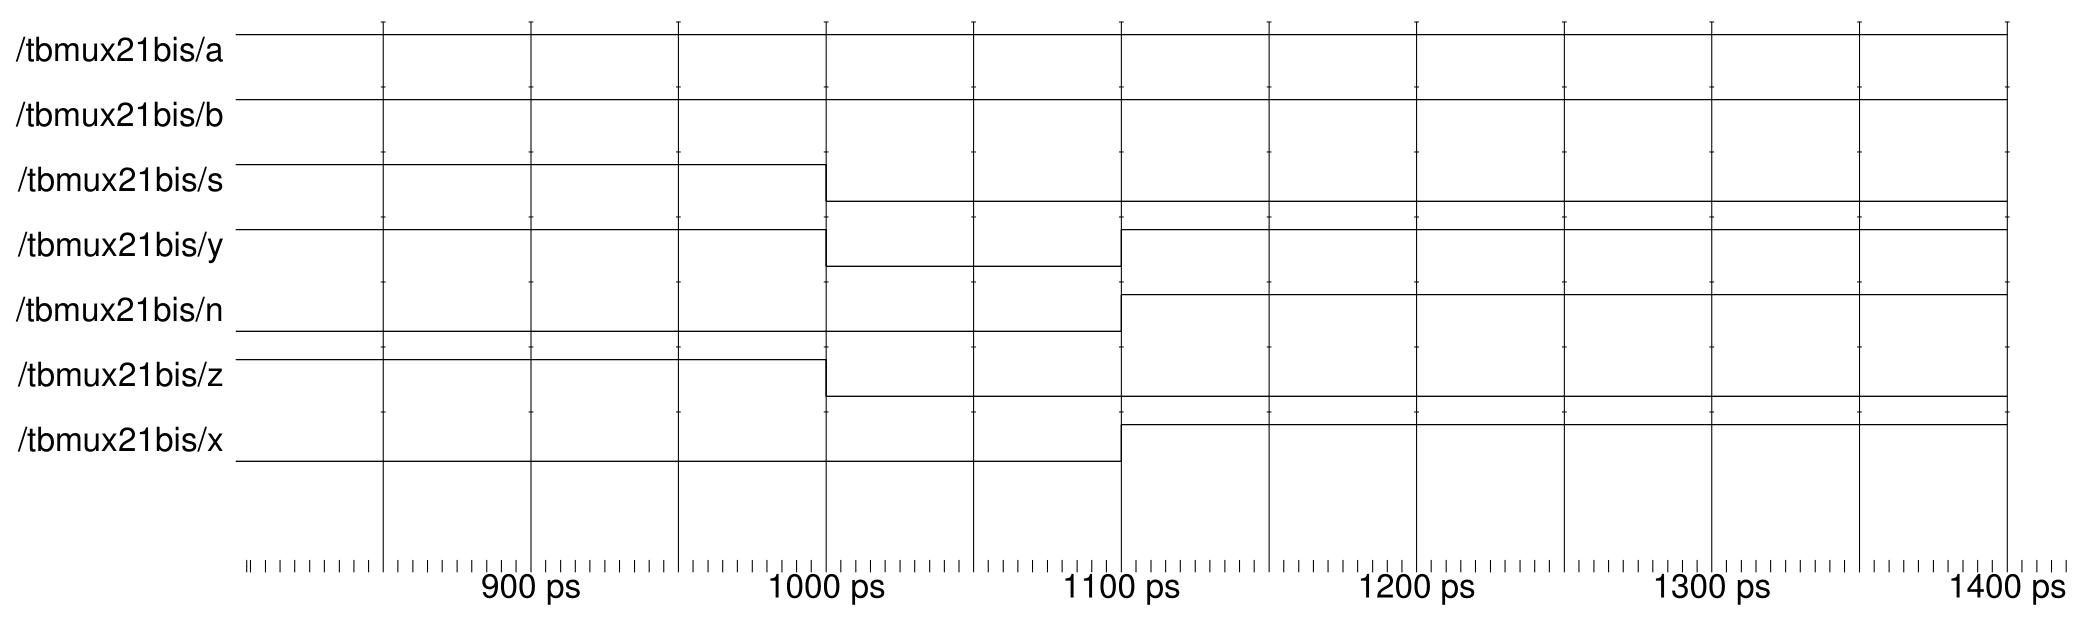
\includegraphics[scale=0.25]{immagini/model_mux}
	\caption{\textit{Power report}}
	\label{model_mux}
\end{figure}
Si può notare benissimo come l'uscita Y abbia un glitch tra 1000 ps e 1100 ps, in quanto effettua una transizione 0->1 non voluta. Il tutto è causato dal ritardo introdotto dall'Inverter, che si può notare dal segnale 'n', che commuta al suo valore corretto dopo un ritardo di 0,1 ns, rispetto all'istante in cui cambiano tutti i restanti gate del circuito, ossia 1000 ps. Si verifica dunque un intervallo di tempo, ossia quello compreso tra 1000 ps e 1100 ps in cui la porta OR ha entrambi gli ingressi bassi e dunque produce un'uscita Y errata. \\
Questo produce quindi un glitch in uscita: in generale i glitch sono problematici a livello di potenza, in quanto si tratta di commutazioni spurie all'interno del mio circuito, che causano uno spreco di potenza. L'energia consumata per ogni doppia commutazione indesiderata è
\begin{center}
	$ E=C_{L}V_{DD}^{2}$
\end{center}
considerando $C_{L}$ come il carico che viene pilotato e $V_{DD}$ la tensione di alimentazione alla quale si lavora. 

\section{Probability and Activity Calculation: Syncronous Counter}
\begin{figure}[!htb]
	\centering
	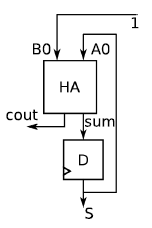
\includegraphics[scale=0.6]{immagini/counter}
	\caption{\textit{Power report}}
	\label{counter}
\end{figure}
\noindent Si analizza in questa sezione un \textit{Syncronous Counter} ad 1 bit, realizzato con una Half Adder e un D-FlipFlop, riportato in Figura \ref{counter}. Il primo ingresso \textit{A0} dell'Half Adder è l'uscita del D-FlipFlop, mentre il secondo ingresso \textit{B0} viene collegato fisso ad 1. Si riporta il timing diagram del circuito in Figura \ref{timing_counter1}.
%%MANCA TIMING DA FARE
Si può dedurre dal timing, che il segnale \textit{S} ha una transizione per ogni colpo di clock, di conseguenza la sua Switching Activity sarà metà dell'attività del segnale di clock. Nel caso in cui il segnale B0 vada a 0, il valore del nodo S dipenderà esclusivamente dall'ultimo valore presente all'uscita del Flip-Flop, in quanto l'Half Adder sommerà l'ultimo valore presente nel Flip Flop con uno '0'. Quindi non si verificheranno più transizioni sul nodo S e di conseguenza neanche sul nodo $C_{OUT}$.
\begin{figure}[!htb]
	\centering
	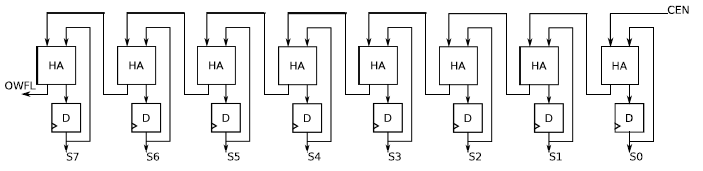
\includegraphics[scale=0.6]{immagini/counter2}
	\caption{\textit{Power report}}
	\label{counter2}
\end{figure}
In seguito viene chiesto di analizzare la struttura presente in Figura \ref{counter2}. Questo circuito permette di ottenere un contatore sincrono ad 8 bit, utilizzando in cascata 8 celle del circuito precedente. Anche in questo si riporta, in Figura \ref{timing_counter2}, il timing diagram del funzionamento del circuito.
%MANCA TIMING
In Tabella \ref{trans_uscita}, vengono ora riportati il numero di commutazioni di tutti i segnali di uscita ricavati in modo analitico, considerando un intervallo di tempo compreso da quando il circuito parte dal valore '00000000', fino a quando non arriva al valore '11111111'.
\begin{table}[!h]\footnotesize
	\centering
	\begin{tabular}{|c|c|}
		\hline
		\textbf{Signal} & \textbf{Number of Transitions}\\
		\hline
		Clock & 511  \\
		S0 &  255 \\
		S1&127\\
		S2& 63\\
		S3& 31\\
		S4& 15\\
		S5& 7\\
		S6& 3\\
		S7& 1\\
		\hline
	\end{tabular}
	\caption{\textit{Risultati simulazione}}
	\label{trans_uscita}
\end{table}\\

Il segnale \textit{CEN}, rappresenta l'enable del contatore, mentre il segnale \textit{OWFL} va ad 1 in presenza di overflow, dunque quando si supera la massima dinamica del contatore. Il segnale CEN è l'ingresso B0 del primo Half-Adder, mentre il segnale OWFL è il carry out dell'ultimo Half-Adder. \\
Il Segnale OWFL farà solo una transizione per ogni ciclo di conta, dunque andrà ad '1', solo quando le uscite S7-S0 andranno dal valore '11111111' al valore '00000000'. Di conseguenza avrò che la Switching Activity sarà:
\begin{center}
	$E_{SW}=\frac{1}{2^{8}-1}=$
\end{center}
Si vuole ora confrontare i risultati analitici ricavati in precedenza ed i risultati ottenuti sfruttando le simulazione di \textit{Synopsis}. In Figura \ref{report_counter}, viene riportata la simulazione ottenuta.\\
\begin{figure}[!htb]
	\centering
	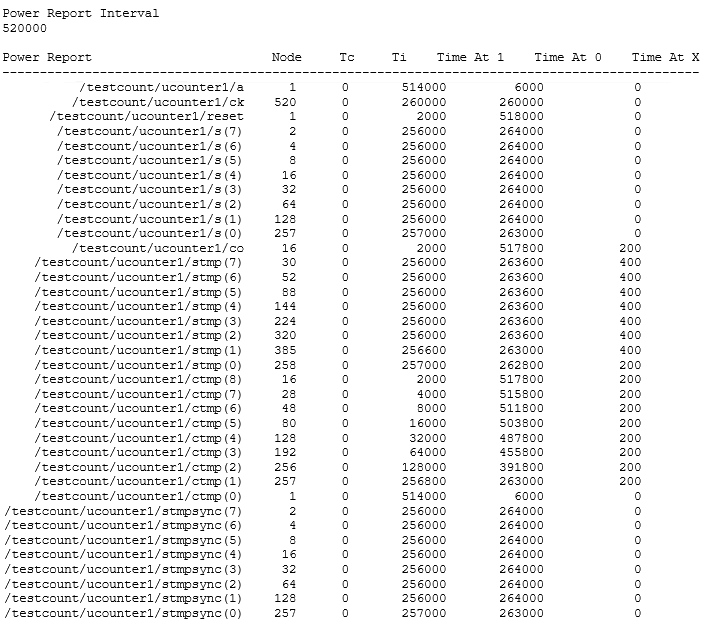
\includegraphics[scale=0.6]{immagini/report_counter}
	\caption{\textit{Power report}}
	\label{report_counter}
\end{figure}
Viene chiesto di confrontare i valori analitici calcolati e riportati nella Tabella \ref{trans_uscita}, con quelli derivanti da una simulazione \textit{Synopsis}. Si simula il comportamento del circuito utilizzando un $T_{CLK}=2 ns$, per un periodo pari a 260 colpi di clock. Il report risultante è presente in Figura \ref{report_counter}.
Andando a studiare i file di testbench riportati, si può notare come vengano introdotti dei ritardi di 0.2 ns nelle uscite dell'Half Adder: questo provoca dei glitch che si andranno a propagare lungo la rete ed avranno effetti sul segnale OWFL, che invece di andare ad '1' solo una volta a fine conteggio, andrà ad '1' per tre volte (DA VERIFICARE!!!).\\
Tramite il power report si può notare come, in generale, il numero di commutazioni della simulazione sia superiore a quello ottenuto analiticamente: si può notare questo fenomeno nei segnali \textit{stmp(n)}, ossia le uscite non sincrone dei Flip Flop, e nei segnali di Carry Out. Il tutto è dovuto ai glitch che si propagano interamente al contatore a causa del ritardo di 0.2 ns di ciascun Half Adder. \\
Fortunatamente, questi glitch vengono filtrati dai Flip-FLop, in quanto il $T_{CLK}$ è superiore al ritardo introdotto dalla rete combinatoria.
